\documentclass{beamer}
\mode<presentation>
\usetheme{CambridgeUS}
\usepackage[russian]{babel}
\usepackage[utf8]{inputenc}
\usepackage[T2A]{fontenc}
\usepackage{sansmathaccent}

\usepackage{verbatim}
\usepackage{alltt}

\pdfmapfile{+sansmathaccent.map}
\title[СУБД]{Структуры базы данных. Часть~1. }
\author{Наумов Д.А., доц. каф. ИТГД, доц. каф. КТ}
\date[28.02.2019] {Основы компьютерных наук (3 часть), 2019}

\begin{document}

%ТИТУЛЬНЫЙ СЛАЙД
\begin{frame}
  \titlepage
\end{frame}
  
%СОДЕРЖАНИЕ ЛЕКЦИИ
\begin{frame}
  \frametitle{Содержание лекции}
  \tableofcontents  
\end{frame}
  
%РАЗДЕЛ 1
\section{Реляционная модель данных}
\begin{frame}{Немного истории}
\begin{itemize}
\item Эдгар Кодд, "Реляционная модель данных для больших совместно используемых банков данных" [1];
\item Основа - теория отношений (XIX век);
\end{itemize}
\begin{block}{Эволюция концепции реляционной модели данных}
\begin{itemize}
\item версия 1, опубликованая в статье в CACM в 1970 г.;
\item версия 2, определена в статье по поводу Тьюринговской премии в 1981 г.;
\item версия 3, доопределена "дюжиной Кодда" — двенадцатью правилами и оценочной системой в 1985 году [2,3];
\item версия 4, определена в опубликованной в 1990 году книге Кодда~[4].
\end{itemize}
\end{block}
\end{frame} 

\begin{frame}{Немного истории}
\begin{block}{Выводы}
\begin{itemize}
\item Существуют два мира с условными названиями "реляционная модель" и "промышленные РСУБД", и эти два мира
пересекаются, но не полностью, создавая, в частности, проблемы переносимости приложений между СУБД разных производителей.
\item Реляционная модель относится к логическим, то есть определённые в рамках модели
структуры, операции над ними и задаваемые ограничения не зависят от способов реализации физической организации данных и управления ими.
\item Каждая СУБД имеет свои особенности физической организации, поэтому одна и та же схема данных в рамках реляционной модели может иметь специфические параметры и опции, оптимизирующие работу с данными.
\end{itemize}
\end{block}
\end{frame} 

\begin{frame}{Определение}
\begin{block}{Отношение}
Для заданных множеств S1, S2, ..., Sn (не обязательно различных) R является отношением на этих n множествах, если представляет собой множество кортежей степени n, у каждого из которых первый элемент взят из множества S1, второй — из множества S2 и т.д. 
\end{block}
\begin{center}
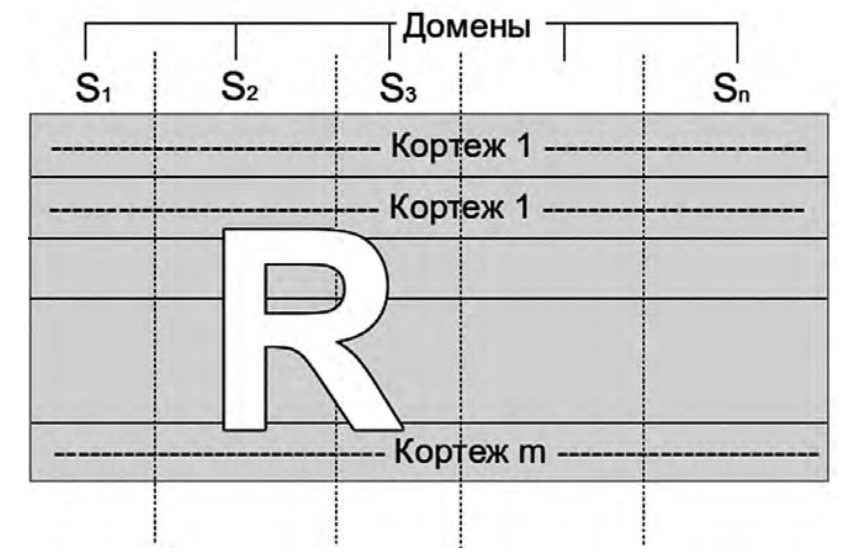
\includegraphics[scale=0.35]{images/rel-01.png}
\end{center}
\end{frame} 

\begin{frame}{Определение}
\begin{block}{Графический смысл отношения}
таблица с зафиксированным типом данных для каждой колонки. 
\end{block}
Реляционные СУБД предлагают своим пользователям оперировать не определениями реляционной алгебры, а их адаптированными аналогами (таблицы, строки, столбцы и т. п.).
\begin{block}{Свойства отношения}
\begin{itemize}
\item в таблице нет двух одинаковых строк;
\item таблица имеет столбцы, соответствующие атрибутам отношения;
\item каждый атрибут в отношении имеет уникальное имя;
\item порядок строк в таблице произвольный.
\end{itemize}
\end{block}
\end{frame}

\begin{frame}{Определение}
\begin{block}{Отношение}
является динамической моделью некоторого объекта реального мира. 
\end{block}
\begin{center}
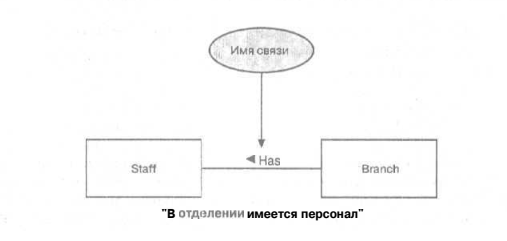
\includegraphics[scale=0.35]{images/rel-02.png}
\end{center}
\begin{block}{Схема отношения}
перечень атрибутов данного отношения с указанием домена, к которому они относятся. 
\[ S_{R} = (A_{1},A_{2},A_{3},..,A_{n}), A_{i} \subset D_{i} \]
\end{block}
\begin{block}{Экземпляр отношения}
отражает состояние данного объекта в текущий момент времени. 
\end{block}
\end{frame}

\begin{frame}{}
\begin{block}{Преимущества реляционной модели данных}
\begin{itemize}
\item теоретическая основа. Формально определяет базовые понятия
модели, язык описания и операции над отношениями;
\item стандартизация. Стандарты SQL-NN (SQL-89, SQL-92, SQL-99 и
т. д.), имеющие несколько уровней полноты реализации, позволяют
создавать приложения, переносимые между СУБД разных
поставщиков;
\item полное разделение доступа к данным от способа их физической
организации;
\item универсальность. Информационное моделирование сущностей
реального мира в виде набора связанных таблиц является достаточно
хорошим подходом в большинстве случаев;
\item простота манипуляции данными с точки зрения конечного
пользователя;
\item SQL — развитый стандартизованный декларативный язык 4-го
поколения.
\end{itemize}
\end{block}
\end{frame}

\begin{frame}{}
\begin{block}{Недостатки реляционной модели данных}
\begin{itemize}
\item в общем случае, более низкое быстродействие по сравнению с
сетевыми и иерархическими СУБД или другими подходами,
обеспечивающими доступ к данным непосредственно на уровне их
физической организации, например, индексированные файлы;
\item неполнота реализации стандартов SQL-NN, а также
специфические языковые и процедурные расширения СУБД разных
поставщиков, осложняющие переносимость приложений (так
называемый vendor lock);
\item необходимость учёта некоторых особенностей модели на
концептуальном уровне (ключи — идентификаторы сущностей),
отсутствующая, например, в сетевой модели.
\end{itemize}
\end{block}
\end{frame}

\section{Другие подходы и модели данных}
\subsection{Модель Сущность-Атрибут-Значение}
\begin{frame}
\begin{block}{САЗ (Сущность-Атрибут-Значение, EAV (Entity-Atribute-Value))}
подход, заключающийся в максимальном упрощении структуры хранения данных, 
за счет "вертикального хранения атрибутов", что обеспечивает высокую гибкость 
изменения логической схемы данных.
\end{block}
\begin{center}
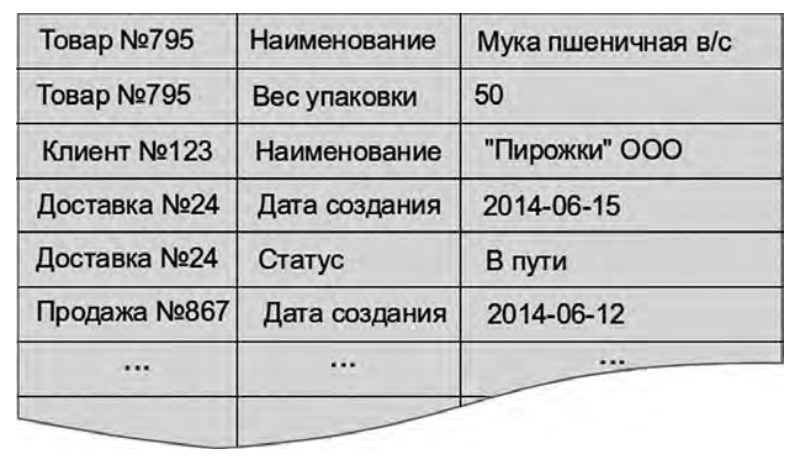
\includegraphics[scale=0.35]{images/eav-01.png}
\end{center}
\end{frame}

\begin{frame}
\begin{center}
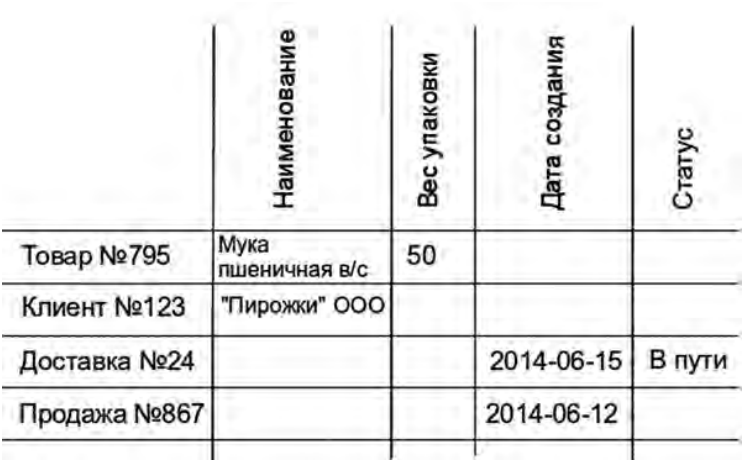
\includegraphics[scale=0.35]{images/eav-02.png}
\end{center}
САЗ даёт возможность менять логическую схему данных, что называется, "на лету".
Действительно, достаточно добавить в метаданные описание нового атрибута и связать его с типами сущностей, как все приложения могут считывать и записывать значения данного атрибута, не принимая во внимание структурные изменения. 
\end{frame}

\begin{frame} 
\begin{block}{Преимущества модели САЗ}
\begin{itemize}
\item гибкость схемы данных и возможность её изменения в динамике;
\item высокая степень унификации и повторного использования структур хранения;
\item возможность выполнения контекстно-независимых запросов, например, не принимающих в расчёт тип сущностей;
\item возможность реализации на основе реляционной СУБД;
\item относительно простая базовая концепция.
\end{itemize}
\end{block}
\begin{block}{Недостатки модели САЗ}
\begin{itemize}
\item сложность манипуляций данными вне CRUD-запросов;
\item необходимость вводить собственный язык манипуляции данными;
\item более низкая производительность за счёт большего числа соединений в запросах;
\item необходимость оптимизации физического хранения.
\end{itemize}
\end{block}
\end{frame} 

\subsection{Неполно структурированные модели данных}
\begin{frame} 
\begin{block}{Неполно структурированные модели данных}
(НСМД, semi-structured data models) - способы организации данных, в которых схема и данные не разделены.
\end{block}
Случаи применения:
\begin{itemize}
\item исходные данные неполно структурированы, а возможности по их анализу и классификации ограничены;
\item обмен информацией в гетерогенной среде.
\end{itemize}
\begin{center}
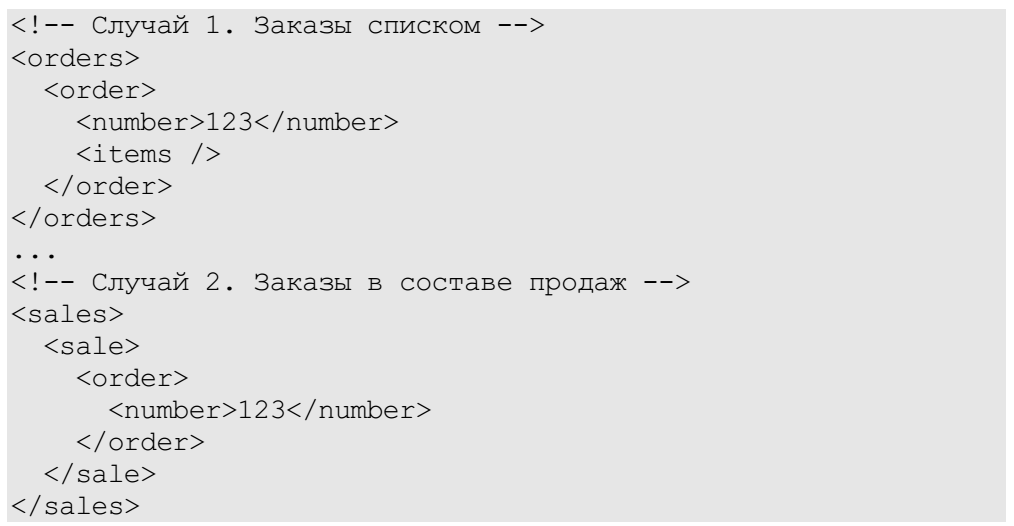
\includegraphics[scale=0.30]{images/xml-01.png}
\end{center}
\end{frame}

\begin{frame}{}
\begin{block}{JSON}
JavaScript Object Notation, формат хранения НСМД, менее удобный для восприятия человеком, но более прост для обработки анализаторами и более экономичный.
\end{block}
\begin{center}
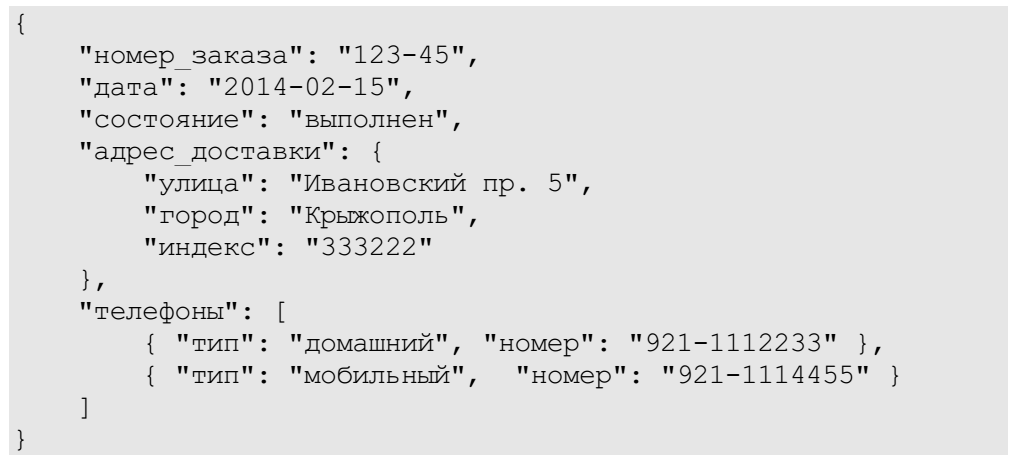
\includegraphics[scale=0.35]{images/json.png}
\end{center}
Концепция самодокументированных данных: информация передаётся между
системами в НСМД, при этом структура считается самодостаточной для распознавания и интерпретации смысловых и контекстных связей в документе без предварительного согласования схем данных для обмена.
\end{frame}

\subsection{Документ-ориентированные модели данных}
\begin{frame} 
\begin{block}{В документ-ориентированной модели данных (ДОМ)}
основным элементом являются документы, организованные в линейные списки — коллекции, которые могут
содержать другие коллекции.
\end{block}
\begin{itemize}
\item В отсутствии строгого определения, понятие "документ" соответствует иерархическим
XML, JSON-документам и подобным структурам.
\item ДОМ представляет собой синтез иерархической и неполно-структурированной моделей данных.
\end{itemize}
СУБД, реализующие документ-ориентированную модель, получили название NoSQL.
\begin{block}{Реализации NoSQL СУБД}
Cassandra, CouchDB, MongoDB.
\end{block}
\end{frame}

\begin{frame} 
\begin{block}{Отличия от РМД и сетевой МД}
В отличие от реляционной модели, где каждая строка таблицы имеет строго оговорённое число полей, определяемых заданными колонками и их типами, или от канонической иерархической модели, где каждый сегмент содержит список записей одного типа, документы списка в ДОМ могут иметь структуру с общей и различающимися частями.
\end{block}
\begin{center}
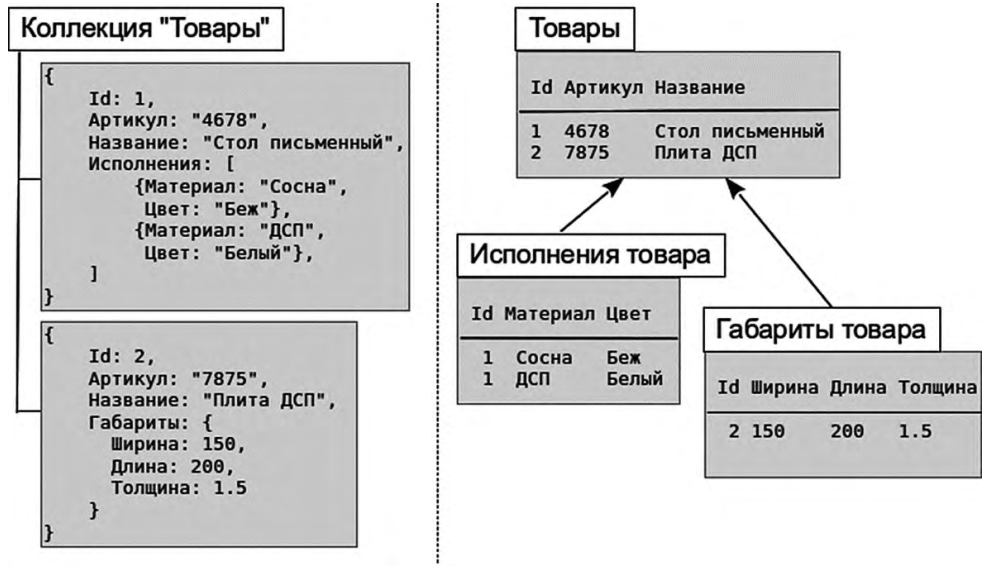
\includegraphics[scale=0.35]{images/dom-01.png}
\end{center}
\end{frame}

\begin{frame} 
Слабым звеном NoSQL является отсутствие стандартизованного декларативного языка запросов.
\begin{center}
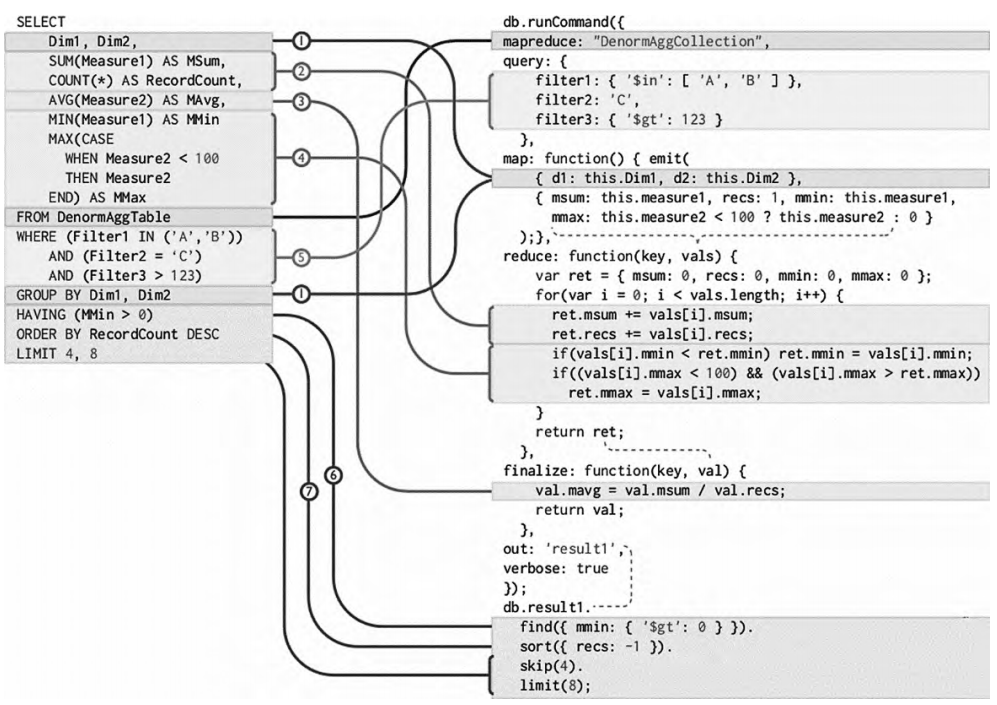
\includegraphics[scale=0.35]{images/nosql-01.png}
\end{center}
\end{frame}

\begin{frame} 
\begin{itemize}
\item Существует класс задач сбора, хранения и первичной обработки неполно структурированной информации, где продукты данного типа могут быть рассмотрены в качестве альтернативы реляционным СУБД, не имеющих
соответствующих расширений для работы с XML или JSON. 
\item Некомпетентность в SQL и реляционных СУБД не может служить серьёзным доводом в выборе NoSQL СУБД.
\end{itemize}
\end{frame}
 
\section*{Литература}
\begin{frame}   
Рекомендуемая литература:
\begin{enumerate}
\item Эдгар Кодд, Реляционная модель данных для больших совместно используемых банков данных. Перевод Communications of the ACM, Volume 13, Number 6, June, 1970. — Журнал "СУБД", №1/1995;
\item Codd, E.F. Is Your DBMS Really Relational?; Computerworld, October 14th, 1985.
\item Codd, E.F. Does Your DBMS Run By The Rules?; Computerworld, October 21st, 1985.
\item Codd, E.F. The Relational Model For Database Management Version 2. Reading, Mass.: Addison-Wesley, 1990.
\end{enumerate}
\end{frame}

\end{document}
